\addcontentsline{toc}{chapter}{Appendix A: State-space}  
\section*{Appendix A: State-space}


% \begin{figure}[ht]
    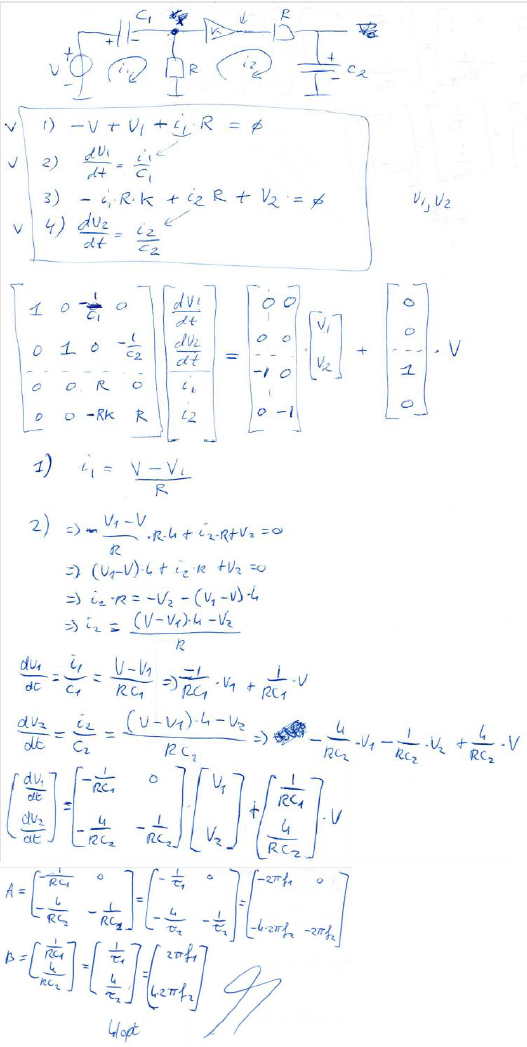
\includegraphics[width=\linewidth, height=\textheight, keepaspectratio]{State-space_notation_solution.png}
%    \caption{State-space notation derived from band-pass filter circuit}
%     \label{fig:state-space-derived-bpf}
% \end{figure}
\newpage
\newpage

\section*{Appendix B: Buck converter schematic}
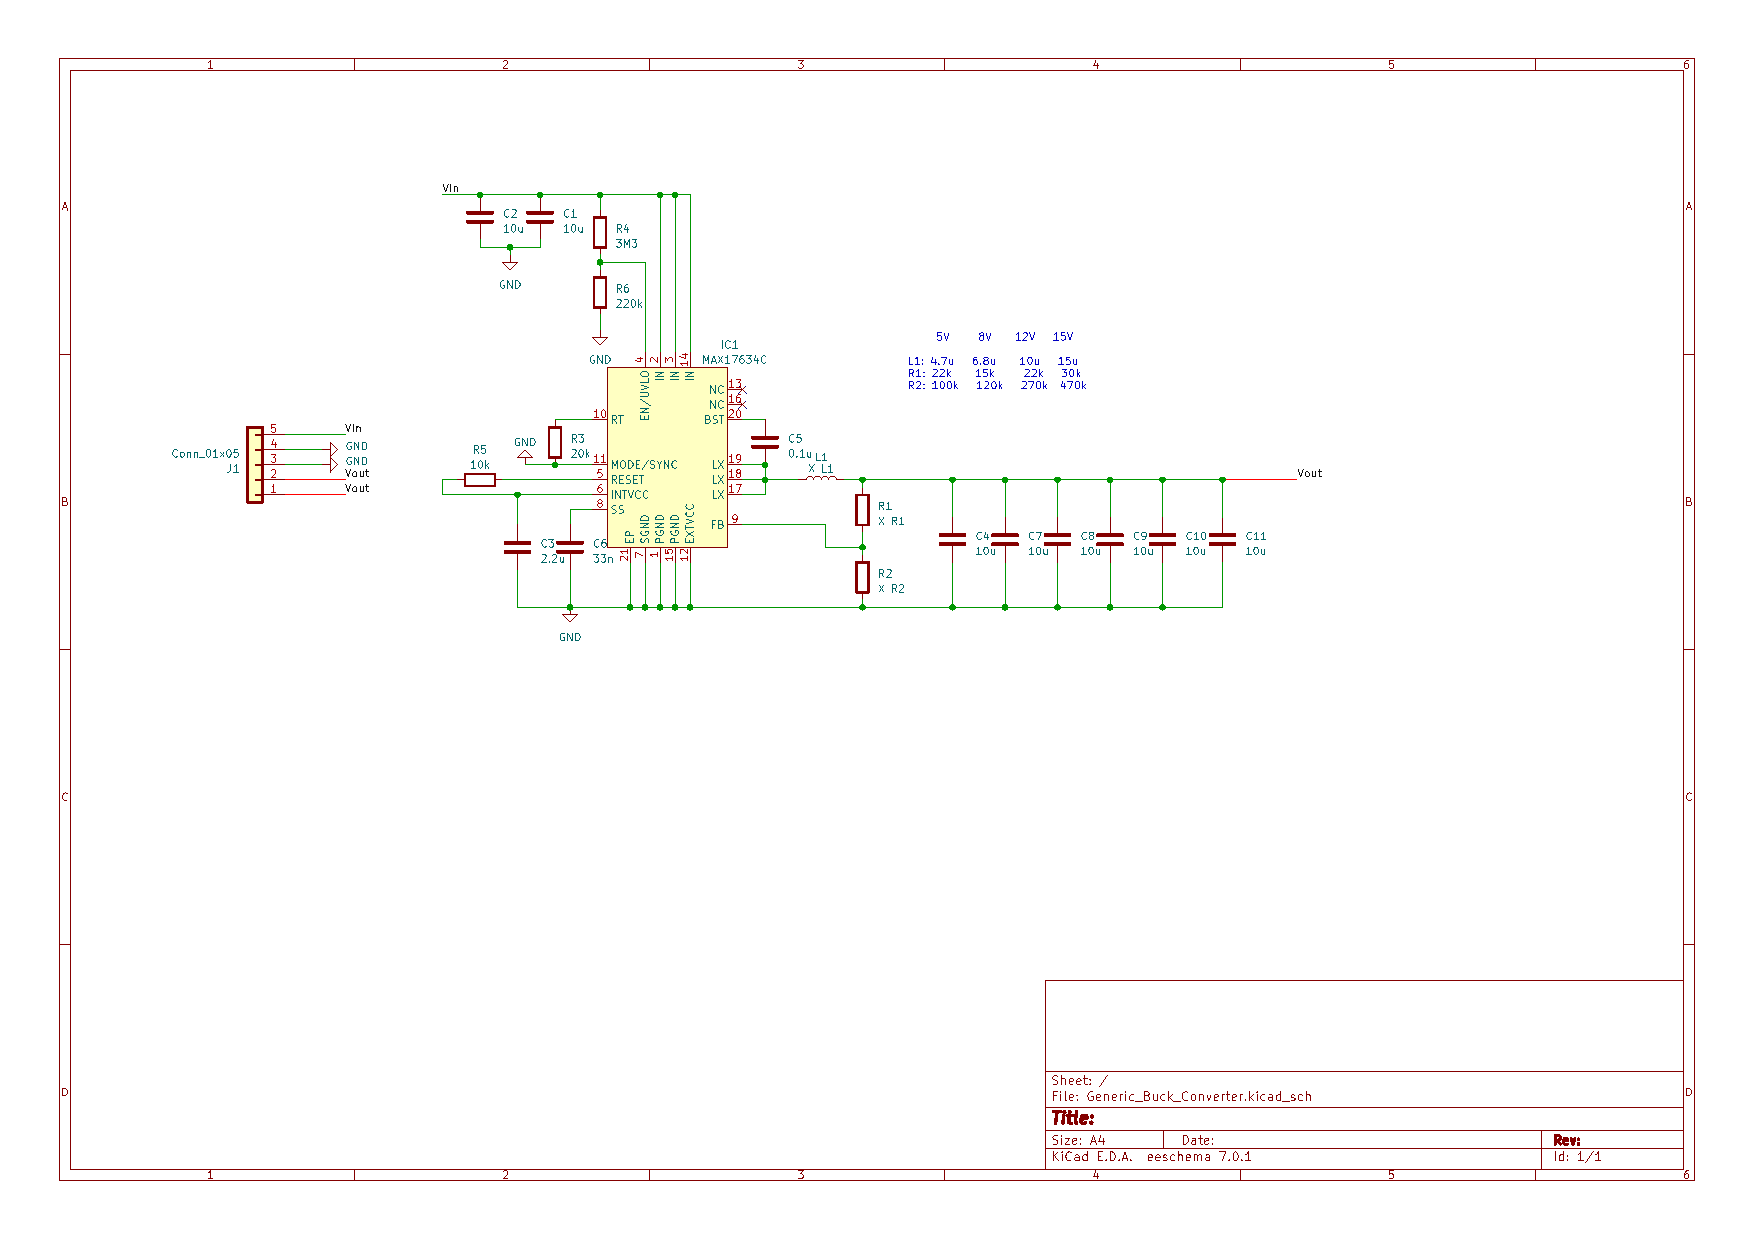
\includegraphics[angle=90, width=500pt]{Generic_Buck_Converter_schematic.pdf}

\section*{Appendix C: SEPIC schematic}
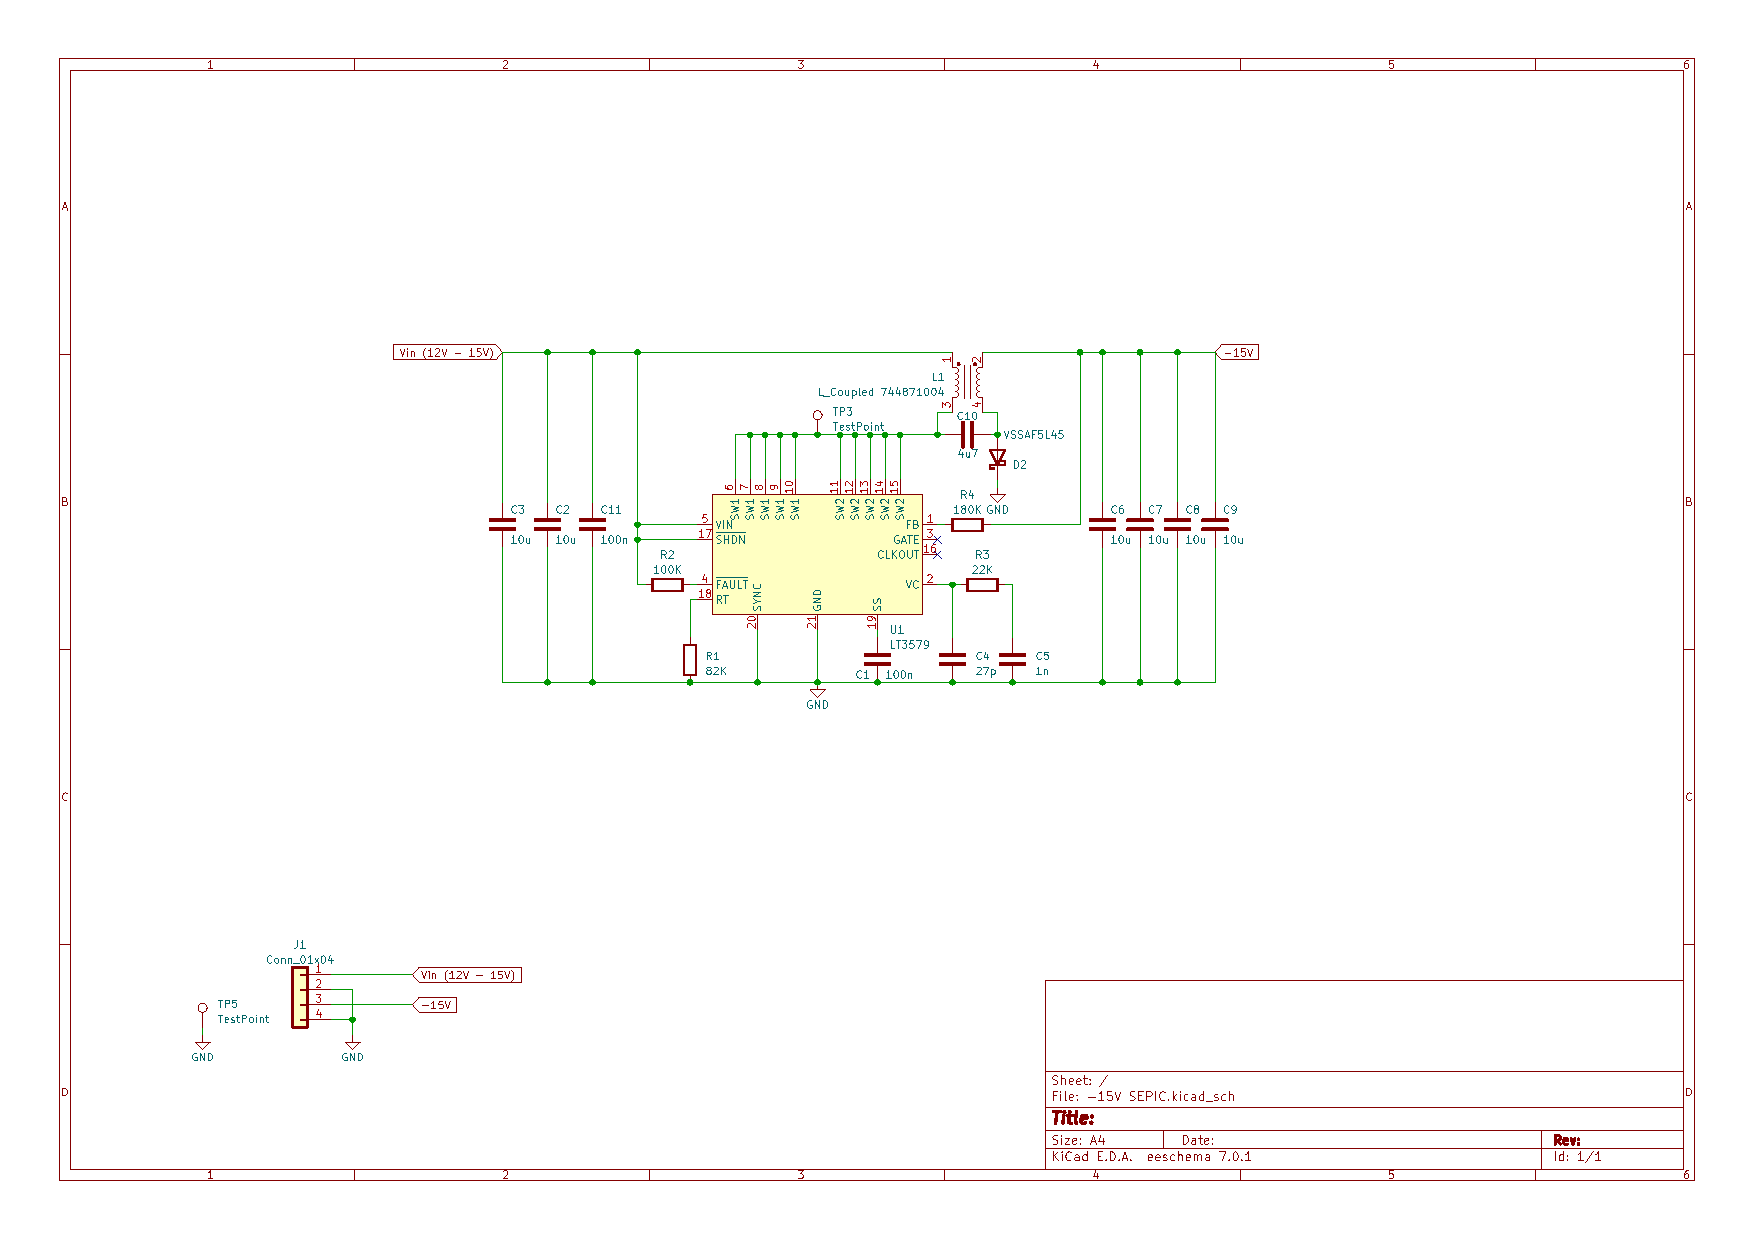
\includegraphics[angle=90, width=500pt]{-15V_SEPIC_schematic.pdf}

\section*{Appendix D: Linear regulator schematic}
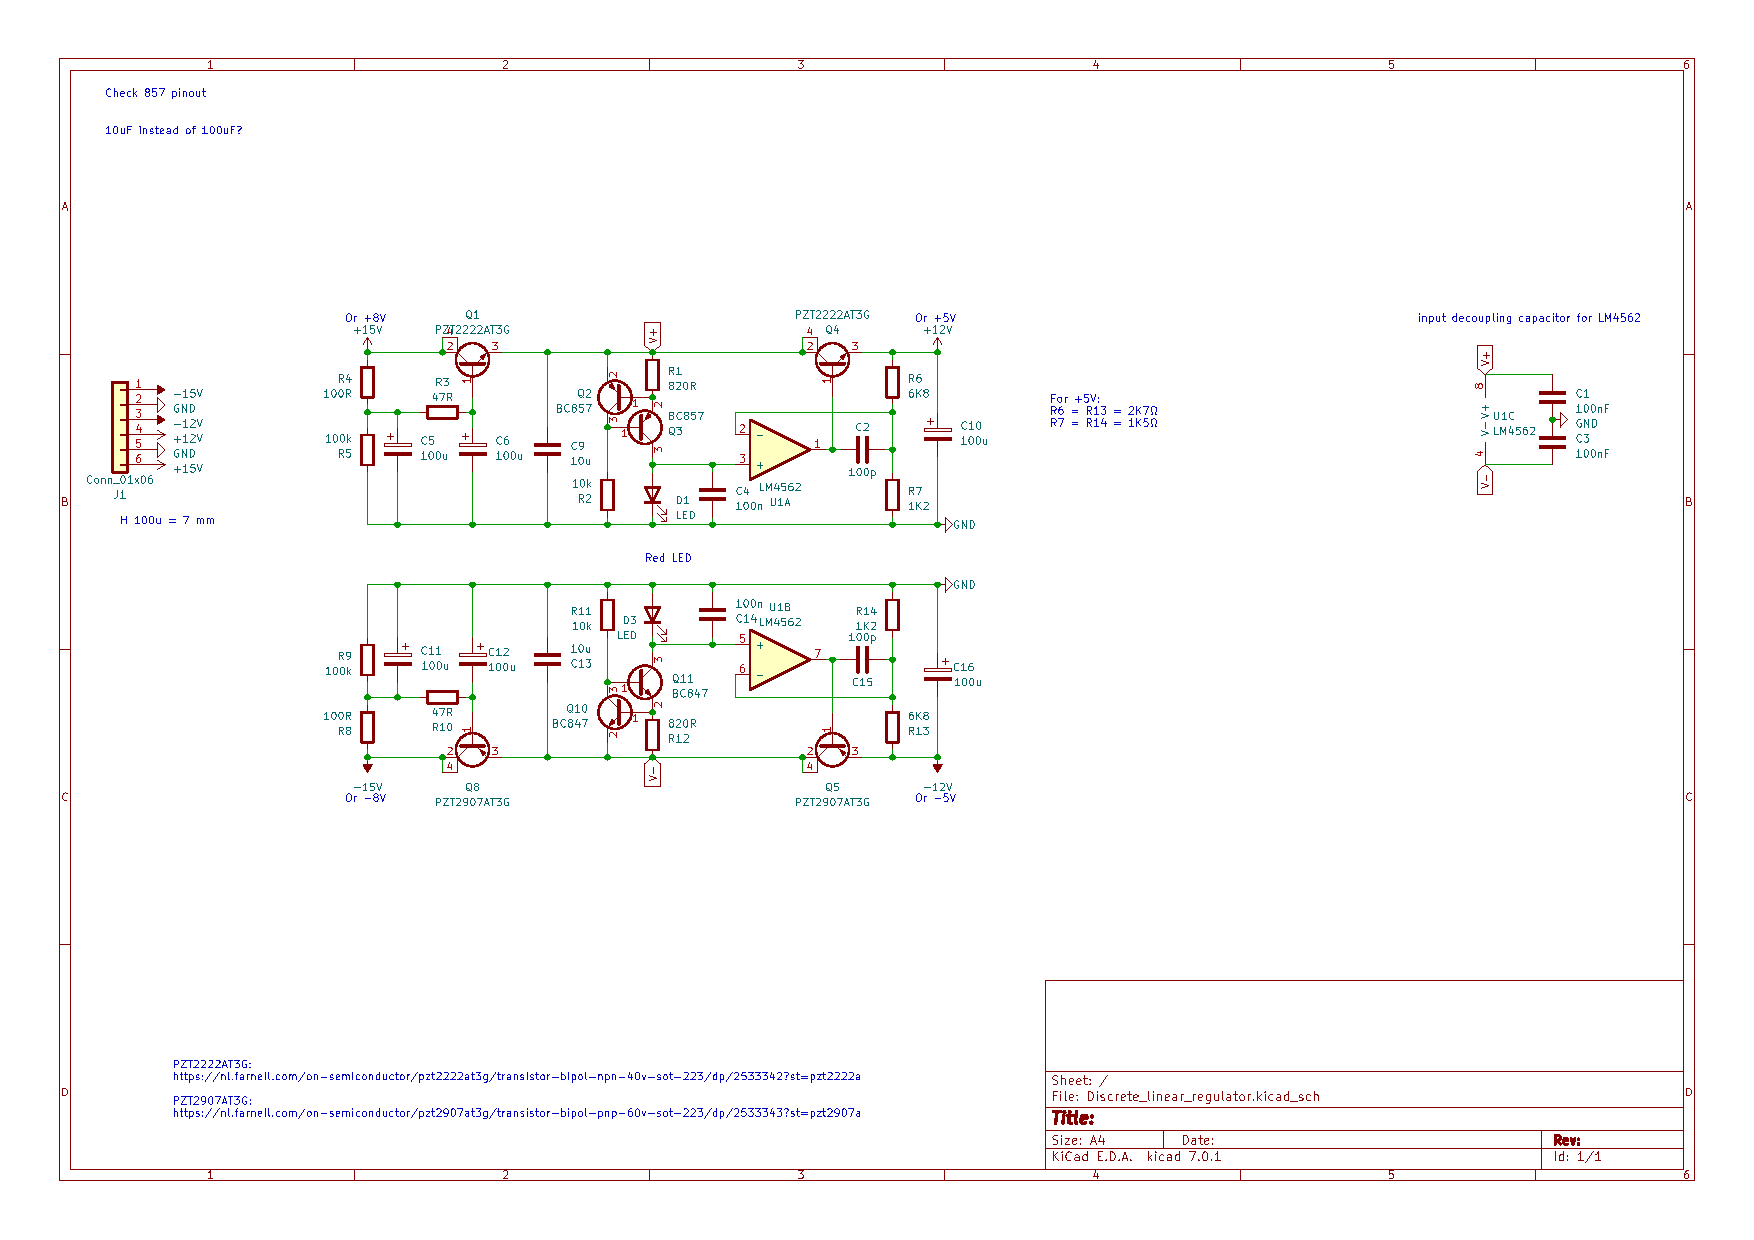
\includegraphics[angle=90, width=500pt]{Discrete_linear_regulator_schematic.pdf}

\section*{Appendix E: Main board schematic}
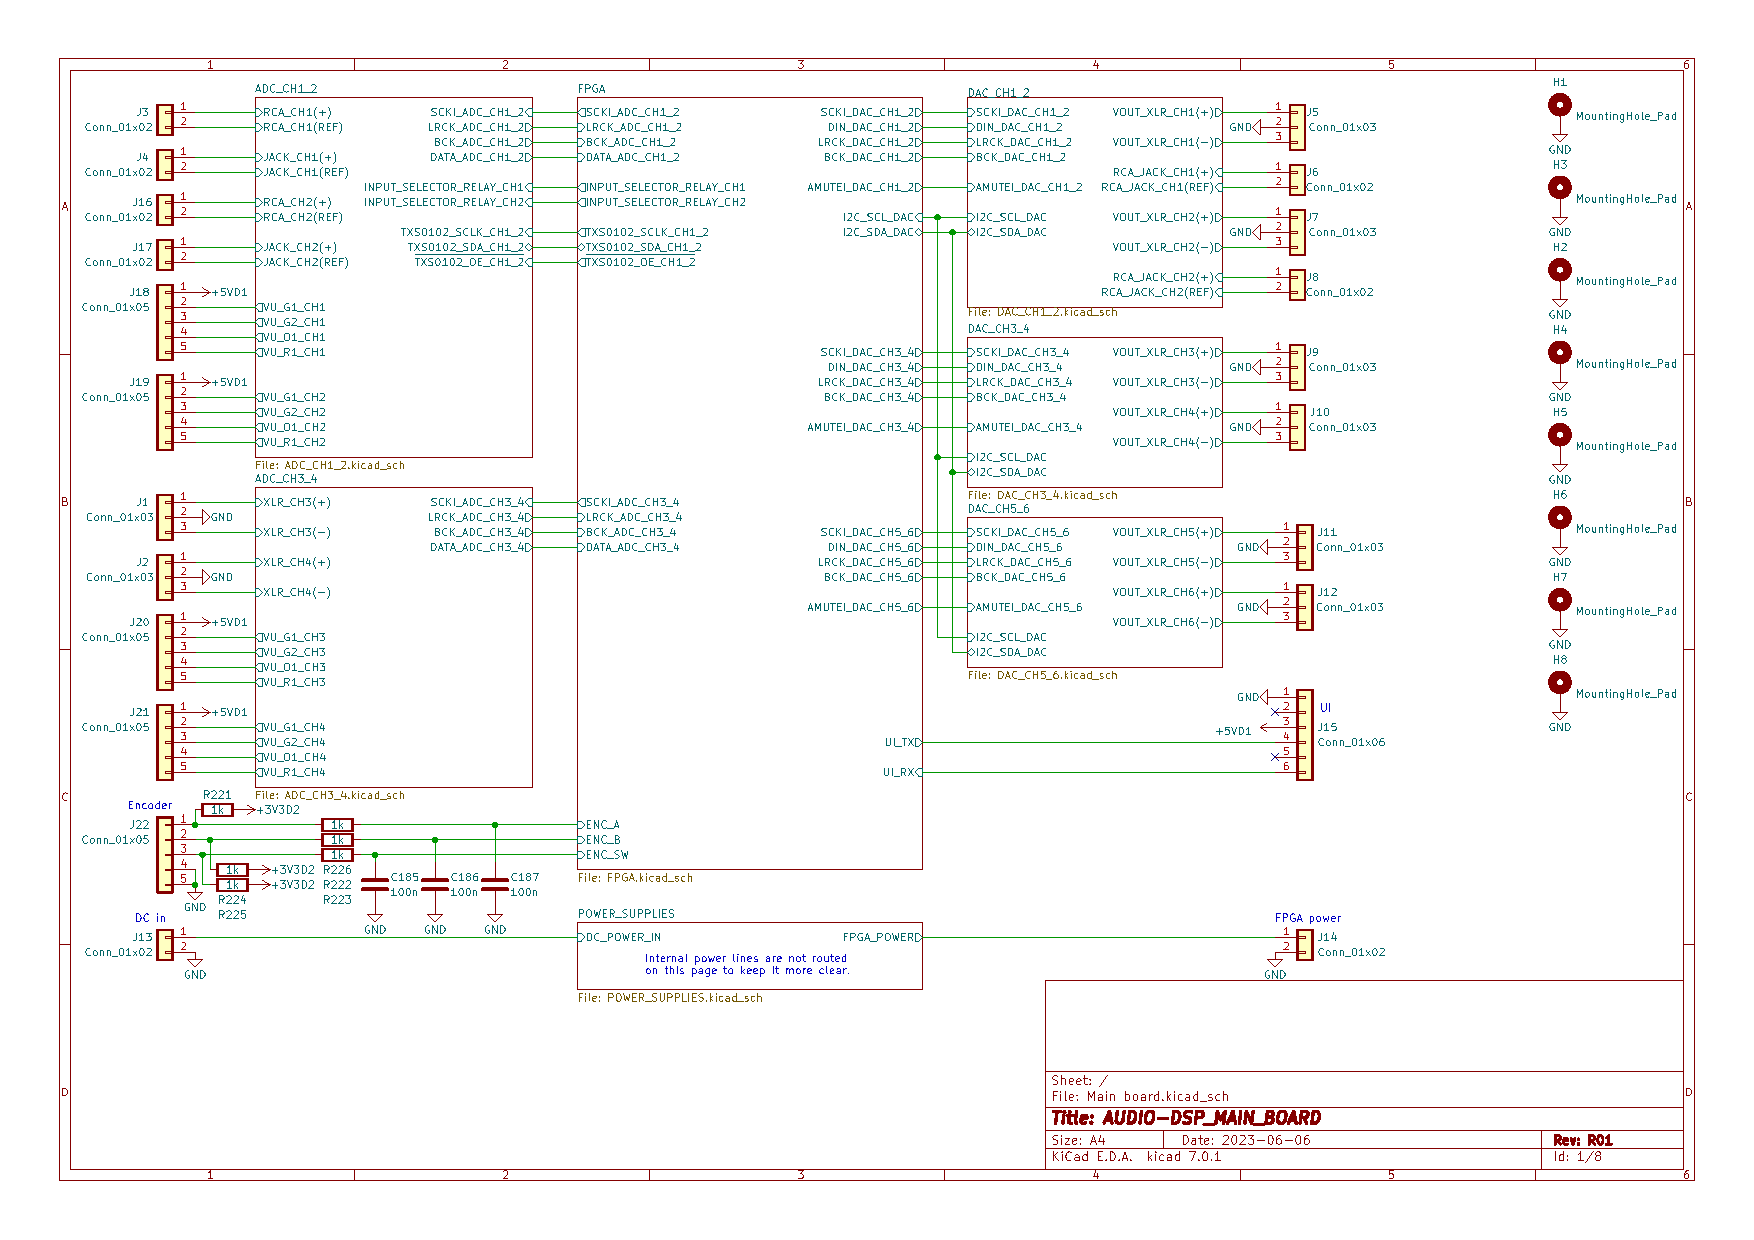
\includepdf[angle=90, pages=-]{Main_board_schematic.pdf}

\section*{Appendix F: UI design} \label{AppendixF}
\begin{figure}[ht]
    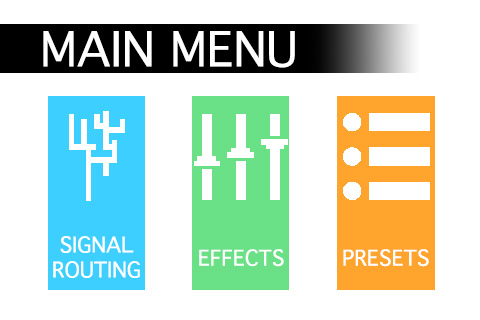
\includegraphics[width=0.7\textwidth]{MainMenu1}
    \caption{Main menu design}
    \label{fig:mainmenu}
\end{figure}

\begin{figure}[ht]
    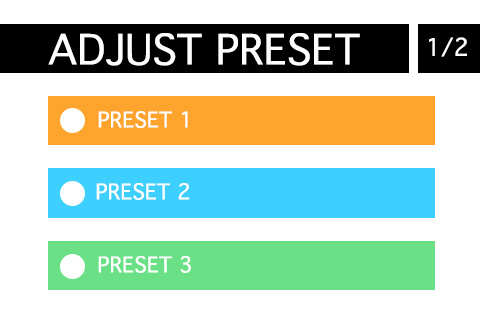
\includegraphics[width=0.7\textwidth]{adjustpreset1-2}
    \caption{Other menu screen, other ones are similar to this one}
    \label{fig:adjustpresetmenu}
\end{figure}

\newpage

\section*{Appendix G: Case} \label{AppendixG}
\begin{figure}[ht]
    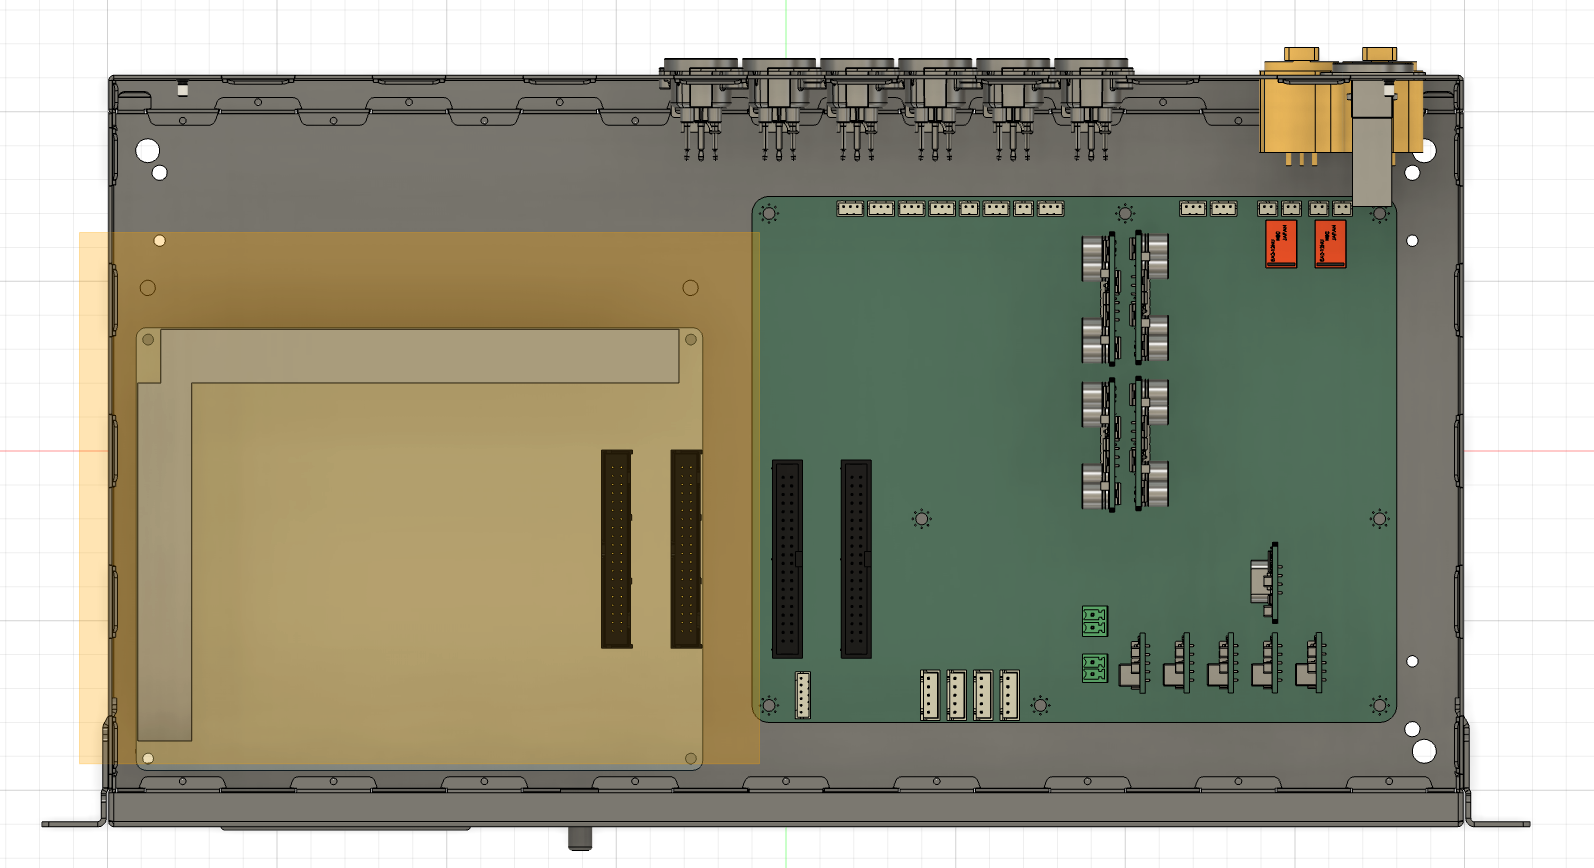
\includegraphics[width=0.8\textwidth]{topviewcase}
    \caption{Top-down view of the case}
    \label{fig:topview}
\end{figure}

\begin{figure}[ht]
    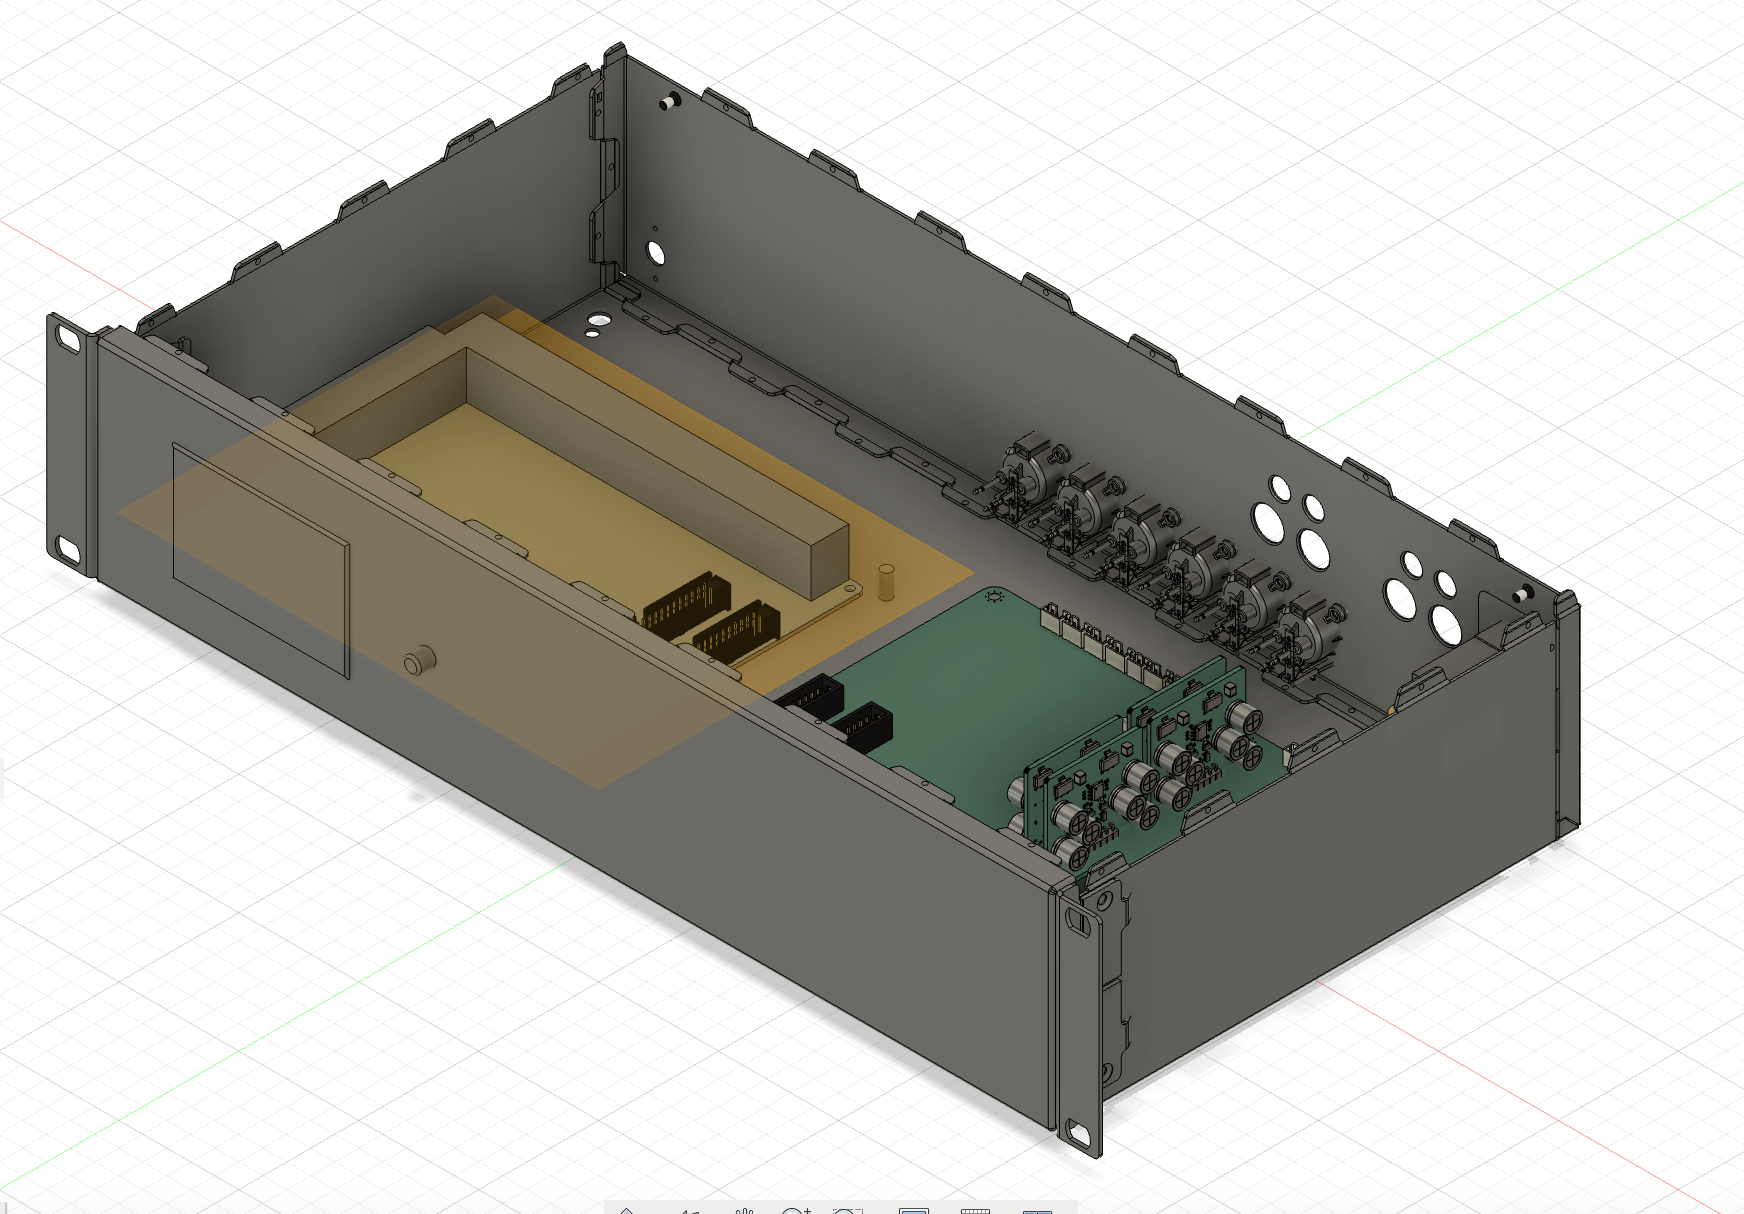
\includegraphics[width=0.8\textwidth]{frontviewcase}
    \caption{Front view of the case}
    \label{fig:frontview}
\end{figure}

\begin{figure}[ht]
    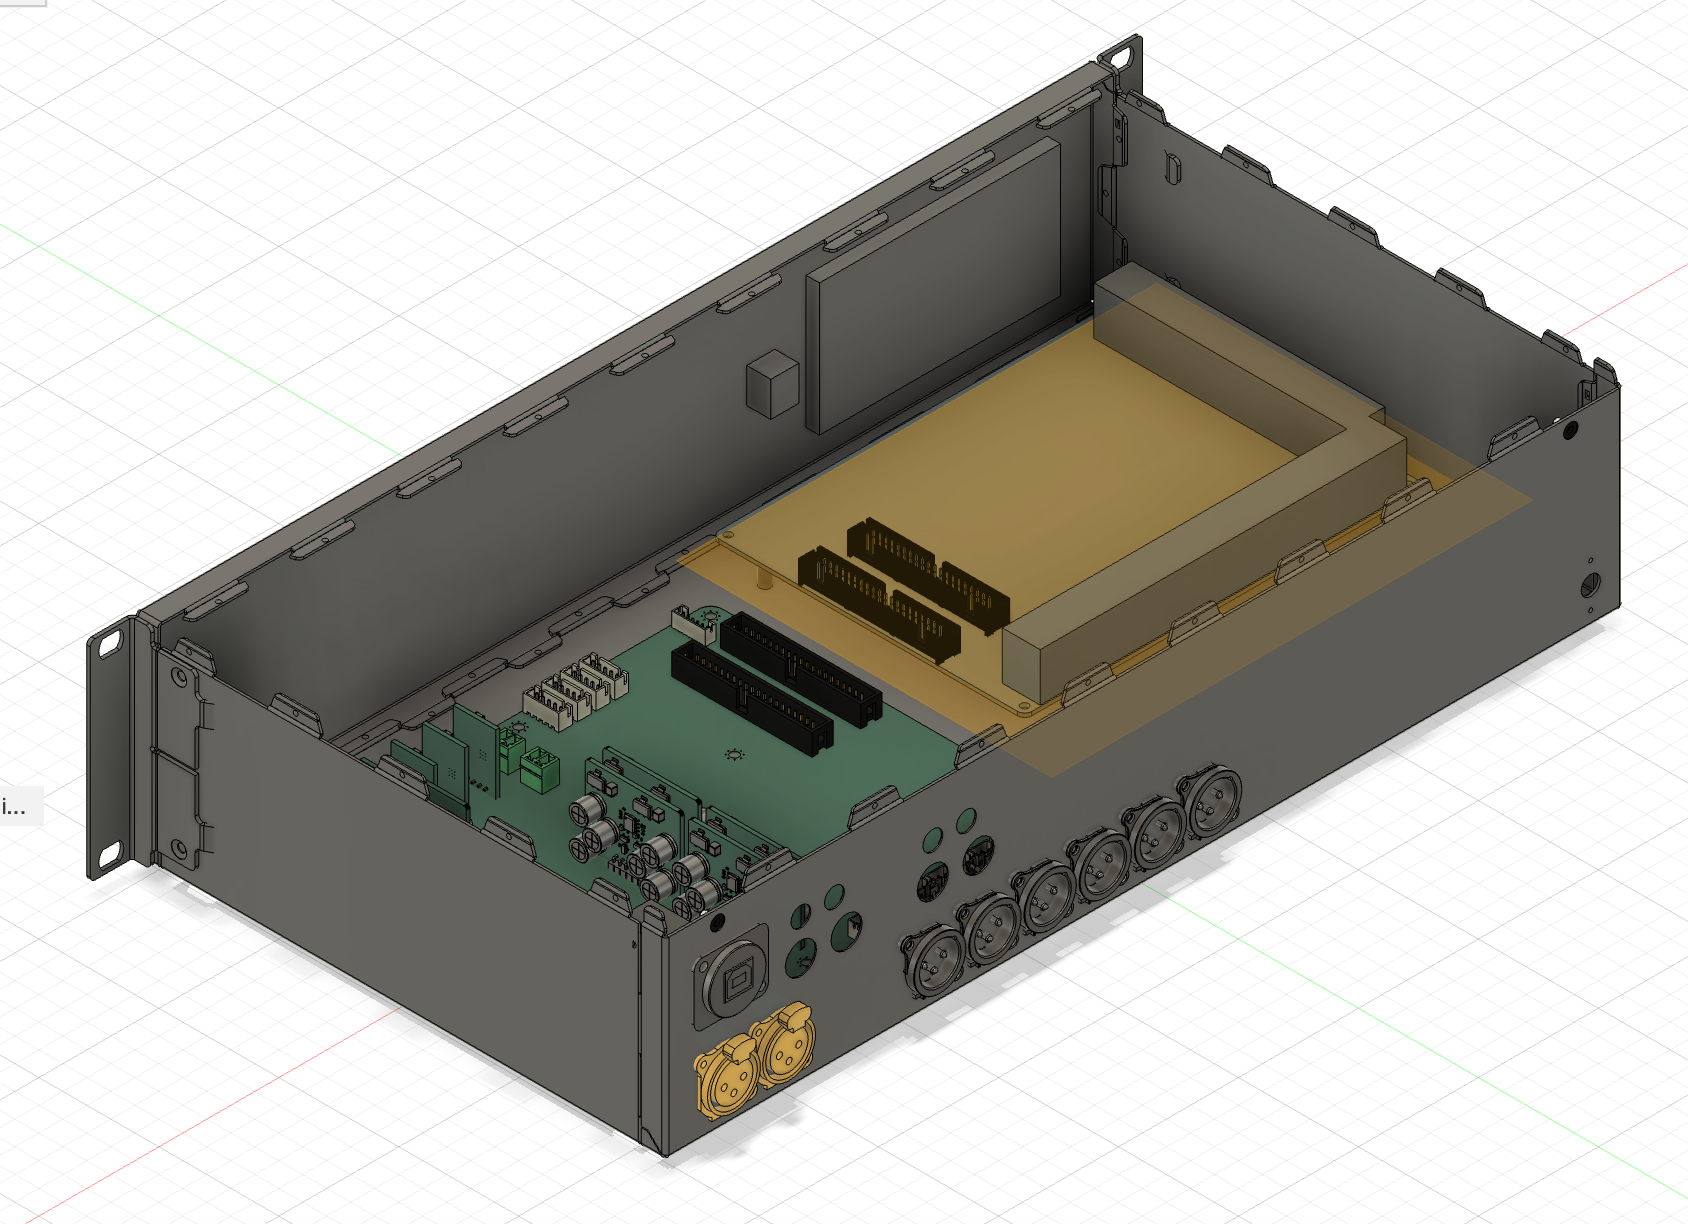
\includegraphics[width=0.8\textwidth]{rearviewcase}
    \caption{Rear view of the case}
    \label{fig:rearview}
\end{figure}

\newpage

